\chapter{Data Representation}


\section{Introduction to Text}
Everything on your computer, from your essays and photos to the songs on
your playlist, is stored as a long list of 0s and 1s. This chapter shows
how: how text, whole numbers, decimals, and compressed files all become
bits.

In computer systems, text is represented in files as a sequence of
characters, each of which corresponds to a specific number, known as a
character code. \index{character code}These character codes are then stored in the file as
binary data.\index{text}

\subsection{Newlines and Carriage Returns}

Two of the character codes that have special meanings are the newline
(often represented as '\textbackslash n') and the carriage return
(often represented as '\textbackslash r').

The newline character signifies the end of a line of text and the
beginning of a new one. If you parse a text file with a Python script, it will see your 'enter' key press as a new line symbol. 
The carriage return character moves the cursor
to the beginning of the line. The use of these characters can vary
between operating systems. Unix-based systems (like Linux and MacOS)
use the newline character to indicate the end of a line, while Windows
systems use a combination of a carriage return and a newline
('\textbackslash r\textbackslash n').
\index{newline}\index{carriage return}
\subsection{ASCII}

The American Standard Code for Information Interchange (ASCII) is one
of the earliest character encodings. It uses 7 bits to represent each
character, allowing it to define up to $2^7 = 128$ different
characters. These include the English alphabet (in both lower and
upper cases), digits, punctuation symbols, \index{control characters}control characters (like
newline and carriage return), and some other symbols.
\index{ASCII}
\subsection{UTF-8}
\index{UTF-8}
UTF-8 (8-bit Unicode Transformation Format) is a \index{variable-width encoding}variable-width
character encoding that can represent every character in the \index{Unicode}Unicode
standard, yet remains backward-compatible with ASCII. For the ASCII
range (0-127), UTF-8 is identical to ASCII. However, it can use additional
bytes (up to 4 bytes in total) to represent characters that are not
included in ASCII, such as characters from other languages, emojis,
and many other symbols. This has made UTF-8 a widely used encoding in
many modern systems.


\section{Alphabets and Accents}
Software developers often encounter
text from diverse languages and cultures. As a developer, it is
crucial to have a solid understanding of alphabets and accents to
effectively handle and process multilingual text. Alphabets, the
building blocks of written language, vary widely across different
nations and regions. Meanwhile, accents, diacritical marks, and other
phonetic notations play a crucial role in conveying the correct
pronunciation and meaning of words.\index{Alphabets} \index{Accents} \index{Diacritical Marks}

Alphabets are sets of letters or symbols used to represent the sounds
of a language. While the Latin alphabet is widely used in many Western
languages, numerous other alphabets exist, such as \index{Cyrillic}Cyrillic, Greek,
Arabic, Devanagari, and Chinese characters. Each alphabet has its own
unique set of letters, often organized in a specific order, and may
include uppercase and lowercase variations.

Accents and diacritical marks are additional symbols added to letters
to modify their pronunciation or provide additional phonetic
information. Accents can appear above, below, or beside a letter, and
they can change the sound, stress, or intonation of a word. For example, in French, the \index{acute accent}acute accent in \'e marks the sound /e/, as in \emph{caf\'e}, while the grave accent in \`e marks the sound /ɛ/, as in \emph{p\`ere}.

When working with multilingual text, it is essential to consider
various factors:

\begin{enumerate}
  
\item \index{character encoding}Character encoding: Different alphabets require specific
  character encodings to represent their letters digitally. Commonly
  used character encodings include ASCII, Unicode, and
  UTF-8. Understanding the appropriate encoding for each language is
  crucial to ensure proper text rendering and avoid data corruption.

\item Text input and validation: Building applications that handle
  user input requires robust text validation. Account for the diverse
  set of characters and possible accents that may appear in
  user-generated content. Implement proper validation and sanitization
  mechanisms to handle text input securely.

\item \index{collation}Sorting and collation: Sorting text from different languages
  involves considering the specific rules and conventions of each
  alphabet. Some languages may have unique sorting orders, while
  others ignore accents or diacritics when determining the order of
  words. Take into account the appropriate sorting and collation
  algorithms to ensure consistent and accurate results.

\item \index{text normalization}Search and indexing: Efficient search and indexing systems must
  be capable of handling multilingual text. Consider appropriate text
  normalization techniques to account for different character
  representations (e.g., case-insensitive matching, ignoring accents),
  enabling users to find relevant content across languages and
  variations in spelling or diacritics.
\end{enumerate}

\begin{Exercise}[title={Counting Bytes}, label={ex:utf8}]
In UTF-8, ASCII characters take 1 byte, accented Latin letters like
\'e take 2 bytes, most Chinese characters take 3 bytes, and emoji take 4
bytes. How many bytes does the text \texttt{café} take? What about a
message of 10 emoji?
\end{Exercise}
\begin{Answer}[ref={ex:utf8}]
\texttt{c}, \texttt{a}, and \texttt{f} take 1 byte each, and \'e takes 2:
5 bytes for 4 characters. Ten emoji take 40 bytes. (In Python,
\texttt{len("café".encode("utf-8"))} returns 5.)
\end{Answer}

\section{Representing Natural Numbers}\label{chap:hexbinary}
\index{natural numbers}Natural numbers are positive whole numbers, such as 1, 2, 3, and so on. -5 is not a natural
number. $\pi$ is not a natural number. $\frac{1}{2}$ is not a natural
number.

\subsection{Base-10 (Decimal)}
You are used to seeing the natural numbers represented in a \textbf{base-10}
\index{Hindu-Arabic numerals}\newterm{Hindu-Arabic} or the \index{decimal}\newterm{Decimal} numeral system. That is, when you see 2531 you
think ``2 thousands, 5 hundreds, 3 tens, and 1 one.'' Rewritten, this is:

$$2 \times 10^3 + 5 \times 10^2 + 3 \times 10^1 + 1 \times 10^0$$

The \index{radix}\newterm{radix} is the number of different digits a base uses before it needs another place. 
For example, values 0, 1, 2, $\cdots$, 8, 9 are all the values for base-10. 
Once 1 is added to 9, we need to increase the amount of digits in a number. 

In any Hindu-Arabic system, the location of the digits is meaningful:
101 is different from 110; the position of a number indicates its magnitude. Here are those numbers in \index{Roman numerals}Roman numerals:
CI and CX. Roman numerals did not have a symbol for zero at all.
%FIXME should we expand on roman numerals..? could be interesting but not needed?

The Hindu-Arabic system gave us really straightforward algorithms for
addition and multiplication. For addition, you memorized the following table:

\begin{tabular}{ c || c | c | c | c | c | c| c| c| c| c }
 & 0 & 1 & 2 & 3 & 4 & 5 & 6 & 7 & 8 & 9 \\
 \hline
0 & 0 & 1 & 2 & 3 & 4 & 5 & 6 & 7 & 8 & 9 \\
1 & 1 & 2 & 3 & 4 & 5 & 6 & 7 & 8 & 9 & 10 \\
2 & 2 & 3 & 4 & 5 & 6 & 7 & 8 & 9 & 10 & 11\\
3 & 3 & 4 & 5 & 6 & 7 & 8 & 9 & 10 & 11 & 12\\
4 & 4 & 5 & 6 & 7 & 8 & 9 & 10 & 11 & 12 & 13\\
5 & 5 & 6 & 7 & 8 & 9 & 10 & 11 & 12 & 13 & 14\\
6 & 6 & 7 & 8 & 9 & 10 & 11 & 12 & 13 & 14 & 15\\
7 & 7 & 8 & 9 & 10 & 11 & 12 & 13 & 14 & 15 & 16\\
8 & 8 & 9 & 10 & 11 & 12 & 13 & 14 & 15 & 16 & 17\\
9 & 9 & 10 & 11 & 12 & 13 & 14 & 15 & 16 & 17 & 18\\
\end{tabular}

When you multiplied two number together, you simply multiplied each
pair of digits. $254 \times 26$ might look like this:

\begin{tabular} {r c c c c | c}
 & & 2 & 5 & 4 & \\
 & & $\times$ & 2 & 6 & \\
 \hline
& &  & 2 & 4 & $6 \times 4$\\
& & 3 & 0 & & $6 \times 5$ \\
& 1 & 2 & & & $6 \times 2$ \\
& & & 8 & & $2 \times 4$ \\
& 1 & 0 & & & $2 \times 5$\\
+ & 4 & & & & $2 \times 2$\\
 \hline
 & 6 & 6 & 0 & 4 &
 \end{tabular}
 

For multiplication, you memorized this table:

\begin{tabular}{ c || c | c | c | c | c | c| c| c| c| c}
 & 0 & 1 & 2 & 3 & 4 & 5 & 6 & 7 & 8 & 9 \\
 \hline
 0 & 0 & 0 & 0 & 0 & 0 & 0 & 0 & 0 & 0 & 0 \\
 1 & 0 & 1 & 2 & 3 & 4 & 5 & 6 & 7 & 8 & 9 \\
 2 & 0 & 2 & 4 & 6 & 8 & 10 & 12 & 14 & 16 & 18 \\
 3 & 0 & 3 & 6 & 9 & 12 & 15 & 18 & 21 & 24 & 27 \\
 4 & 0 & 4 & 8 & 12 & 16 & 20 & 24 & 28 & 32 & 36 \\
 5 & 0 & 5 & 10 & 15 & 20 & 25 & 30 & 35 & 40 & 45 \\
 6 & 0 & 6 & 12 & 18 & 24 & 30 & 36 & 42 & 48 & 54 \\
 7 & 0 & 7 & 14 & 21 & 28 & 35 & 42 & 49 & 56 & 63 \\
 8 & 0 & 8 & 16 & 24 & 32 & 40 & 48 & 56 & 64 & 72 \\
 9 & 0 & 9 & 18 & 27 & 36 & 45 & 54 & 63 & 72 & 81 
 \end{tabular}

\subsection{Base-2 (Binary)}
\index{binary}\index{base-2}
Binary, on the other hand, has only 2 digits it can have: $0$ or $1$. 
This kind of number system is often used for electrical and computer systems because the values can only be \textbf{on} or \textbf{off}.

Each digit in a binary number represents a power of $2$, starting from the rightmost digit (the least significant bit, or LSB). For example:

\[
  \dots + 2^3 + 2^2 + 2^1 + 2^0
\]
For example,
\[
1011_2 = (1 \cdot 2^3) + (0 \cdot 2^2) + (1 \cdot 2^1) + (1 \cdot 2^0) = 8 + 0 + 2 + 1 = 11_{10}
\]\footnote{The subscripts represent the radix or base.}

Because the radix is 2, the numbers increase differently:
\index{binary!counting in}
\begin{align*}
  0&: 0 \\
  1&: 1 \\
  2&: 10 \\
  3&: 11 \\
  4&: 100 \rightarrow (2^{2}\cdot 1) + 0 + 0 = 4 \\
  5&: 101 \\
  6&: 110 \\
  7&: 111 \\
  8&: 1000 \\
  \cdots& \\
  15&: 1111
  \cdots& \\
\end{align*}

\subsubsection*{Conversion from Decimal to Binary}
To convert $13_{10}$ to binary, repeatedly divide by $2$ and record the remainders until the divisor reaches 0 or 1:
\begin{align*}
13 \div 2 &= 6 \text{ remainder } 1 \\
6 \div 2 &= 3 \text{ remainder } 0 \\
3 \div 2 &= 1 \text{ remainder } 1 \\
1 \div 2 &= 0 \text{ remainder } 1
\end{align*}
Reading from bottom to top, $13_{10} = 1101_2$.

\subsubsection{Bits and Bytes}
A singular binary digit (0 or 1) is called a \newterm{bit}. \index{bit}\index{byte}
A lightbulb, switch, or any sort of \newterm{Boolean} value (true or false) can be represented as a bit.
 
Eight bits form a \emph{byte}, which is a common unit of storage in computer systems:
\[
1\ \text{byte} = 8\ \text{bits}
\]
For example, the binary sequence $01001000$ represents one byte of data.

We will not go into the depths of it here, but here are the basics of computer architecture. 
\index{computer architecture}
Memory is a long list of bytes. \index{memory}
Programs group these bytes into data types:


\index{data types}\textbf{Common Data Types in Memory}

\begin{center}
  
  \begin{tabular}{|c|c|c|c|}
  \hline
  \textbf{Data Type} & \textbf{Size} & \textbf{Bit Length} & \textbf{Typical Use} \\
  \hline
  Character & 1 byte & 8 bits & ASCII characters, small integers \\
  \hline
  Integer & 4 bytes & 32 bits & Whole numbers \\
  \hline
  Double & 8 bytes & 64 bits & Decimal (floating-point) values \\
  \hline
  \end{tabular}
\end{center}


Strings are formed by listing characters in consecutive memory addresses such that they are marked by a starting memory address and ending memory address. 

8-bit binary numbers can be used to signify positive or negative numbers.  \index{signed bits}
The most significant bit (MSB) will alter sign, causing the range to be $[-2^{7}, \; 2^{7}-1]$. \index{two's complement}This scheme is called \newterm{two's complement}. To negate a number, invert every bit and add 1. To read a byte whose MSB is 1, count the MSB as $-128$ instead of $+128$ and add the rest as usual: 

\[
-85_{10} = -1 \times 2^7 + 0 \times 2^6 + 1 \times 2^5 + 0 \times 2^4 + 1 \times 2^3 + 0 \times 2^2 + 1 \times 2^1 + 1 \times 2^0 = 1010 1011
\]

Binary can be easily converted to \newterm{Hexadecimal}. 

\subsection{Base-16 (Hexadecimal)}
\index{hexadecimal}
Hexadecimal (from the Greek \emph{hexa}, meaning six, and the Latin \emph{decem}, meaning ten, which add up to 16) is a representation of number with a radix of 16. Digits are represented through numeric numbers 0-9 and \newterm{A-F}. 

Counting to 16 in hex goes as follows:
\begin{align*}
  &1 \\
  &2 \\
  &3 \\
  &\dots \\
  &9 \\
  &\text{A} \; (\text{decimal value} \;  10) \\
  &\text{B} \; (\text{decimal value} \; 11) \\
  &\text{C} \; (\text{decimal value} \; 12) \\
  &\text{D} \; (\text{decimal value} \; 13) \\
  &\text{E} \; (\text{decimal value} \; 14) \\
  &\text{F} \; (\text{decimal value} \; 15) \\
  &10 \; (\text{decimal value} \; 16)
\end{align*}

Converting between binary and hexadecimal is easy because $16 = 2^4$, so each hex digit matches exactly four binary digits. 

It takes 4 binary digits to represent 1 hex digit: $15 =$ F

For example,
\[0\text{x}47 = 0100 \; 0111_{2}\]
\[0\text{x}\text{BD} = 1011 \; 1101_{2}\]


\subsubsection{Hex Color Codes}
Hex colors are represented by 6 hexadecimal digits, grouped as two each for red, green, and blue (RGB). Each pair ranges from \texttt{00} (0 in decimal) to \texttt{FF} (255 in decimal), allowing 256 shades per color channel. For example:\index{hexadecimal}

$$
\#\text{FF}0000 = \text{Red}, \quad\#00\text{FF}00 = \text{Green}, \quad \#0000\text{FF} = \text{Blue}
$$

By mixing values, you can create millions of unique colors, e.g.:

$$
\#\text{FFA}500 = \text{Orange}, \quad \#800080 = \text{Purple}, \quad \#\text{FFFFFF} = \text{White}, \quad \#000000 = \text{Black}
$$
There are $256^3 = 16{,}777{,}216$ possible color combinations in the RGB hex system. The higher the red, green, or blue values are (closer to 255), the brighter the component becomes and the overall color shifts closer to white. Conversely, the lower the values are (closer to 0), the darker the component becomes and the overall color shifts closer to black.\index{hex colors}

Included in your digital resources are multiple hex videos, as well as an interactive hex color guessing game.

\subsection{Base-8 (Octal)}
\index{Octal}
Octal is another representation of radix 8. Digits range from 0 to 7, and a new digit is added when the count passes 7.

Just as in the above systems, octal increases by the radix —-- powers of 8. For example,

$$
135_{8} = (1 \times 8^2) + (3\times 8^1) + (5\times 8^0) = 64 + 24 + 5 = 93_{10}
$$

\subsubsection{Why Octal Matters}
Octal was historically important in computing because early computers often worked with word sizes that were multiples of 3 bits (such as 12, 24, or 36). Since each octal digit corresponds exactly to 3 binary digits, it was a convenient shorthand for binary values before hexadecimal became more widespread. For example:

$$
110101_2 = 65_8
$$

Even though modern systems mostly use hexadecimal, octal is still used in some contexts, such as Unix file permissions (e.g., \texttt{chmod 755}).


\section{Floating Point Arithmetic}
\subsection{Why Computers Cannot Count Perfectly}

Computers are known to be very precise. Modern processors can perform billions of calculations per second, so it is not intuitive to realize they have this persistent limitation: they cannot store most numbers exactly.

Let us think about what it would actually take to store a number like $\frac{1}{3}$. You
probably know its decimal expansion:
\[
    \frac{1}{3} = 0.3333333\ldots\]
The digits go on forever. Now imagine you are a computer with a fixed amount of memory.
You cannot store infinitely many digits. So you store $0.333$ or $0.3333333$, depending on how much space you have, and you accept that the result is not exactly right. That gap between the number you wanted and the number you
actually stored is called \newterm{approximation error}\index{approximation error}, and
it never fully goes away.

This is not just a problem for fractions with repeating decimals. \index{irrational number}Irrational numbers like
$\sqrt{2} = 1.41421356\ldots$ and \index{transcendental number}transcendental numbers like $\pi = 3.14159265\ldots$
also have infinite, non-repeating decimal expansions. Every one of them must be
approximated when stored in a computer.

To handle this systematically, mathematicians and engineers developed the
\newterm{floating-point system}\index{floating-point system}. Before we look at how it works, it helps to understand the two core reasons why any finite system will always fall short of
the real number line.

\subsubsection{The Number Line is Continuous and Unbounded}

Between any two real numbers, no matter how close together, there are infinitely many
others. Pick any two decimals you like. For example, if you picked $1.00$ and $1.01$, you can always find a number between them: $1.005$, $1.0051$, $1.00500001$, and so on without end. This is referred to as \newterm{continuity}\index{continuity}. A computer's number system cannot be continuous. It stores numbers using a fixed string
of digits, which means it can only represent finitely many values. Real numbers have to be \index{rounding}rounded to the nearest representable value. 

The real numbers stretch infinitely in both directions. There is no largest real number
and no smallest positive real number. A computer's memory is finite, so its number system must have both a largest and a smallest representable value. Numbers too large to store cause a problem called \newterm{overflow}\index{overflow}. Numbers too small to distinguish from zero cause \newterm{underflow}\index{underflow}. 


% Add example
%test edit

\begin{Exercise}[title={Overflow and Underflow}, label={ex:overflow}]
Suppose a floating-point system can only represent numbers between $10^{-4}$ and $10^{8}$.
\begin{enumerate}
    \item Planck's constant is approximately $6.63 \times 10^{-34}$ J$\cdot$s. Does it
    cause underflow, overflow, or neither in this system?
    \item The speed of light is approximately $3.00 \times 10^{8}$ m/s. Does it
    cause underflow, overflow, or neither in this system?
    \item Give one example of a number that would cause overflow.
\end{enumerate}
\end{Exercise}
\begin{Answer}[ref={ex:overflow}]
\begin{enumerate}
    \item Underflow. $6.63 \times 10^{-34}$ is far below $10^{-4}$.
    \item Overflow. $3.00 \times 10^{8}$ is larger than $10^{8}$.
    \item Any number greater than $10^{8}$.
\end{enumerate}
\end{Answer}


So what can we do?

We cannot fix these limitations, because they are baked into the nature of finite computation.
What we can do is design the floating-point system carefully so that the errors it introduces are small, predictable, and manageable. That is exactly what engineers and mathematicians have spent decades working out, and it is what the rest of this chapter is about!

The key insight is that a floating-point number is not just a string of digits. \index{float}A floating-point number has three parts: a \newterm{sign}\index{sign}, a \newterm{significand}\index{significand}
(sometimes called the \index{mantissa}mantissa), and an \newterm{exponent}\index{exponent}.


\subsection{Binary and the Floating-Point System}

In the previous section you saw that computers cannot store most numbers
exactly.
Now the natural question is: how do they store numbers at all?
The answer starts at the hardware level, with the smallest possible piece of
information a computer can hold.

\subsubsection{Binary System}

Every process inside a CPU comes down to the flow of electrical current through
tiny switches called \newterm{transistors}\index{transistors}.
A transistor is either on (carrying current) or off (not carrying current).
That gives us exactly two states, which we write as $0$ and $1$.
This is why computers use \newterm{binary}\index{binary}: it is the only number
system that hardware can physically implement with a simple on/off switch.

A single binary digit is called a \newterm{bit}\index{bit}.
Eight bits grouped together form a \newterm{byte}\index{byte}.
You have probably seen units like megabyte (MB) or gigabyte (GB) before.
One \index{megabyte}megabyte is $10^6$ bytes, and one gigabyte is $10^9$ bytes.
A modern smartphone holds tens of billions of bits.

\begin{Exercise}[title={Bits and bytes}, label={ex:bits-bytes}]
  \begin{enumerate}
    \item A file is $4$ megabytes.
          How many bytes is that?
          How many bits?
    \item A hard drive stores $500$ gigabytes.
          How many bits can it hold?
          Write your answer using scientific notation.
    \item A single bit can be $0$ or $1$.
          Two bits together can be $00$, $01$, $10$, or $11$, which are four possible
          values.
          How many distinct values can $8$ bits (one byte) represent?
          How about $64$ bits?
  \end{enumerate}
\end{Exercise}
\begin{Answer}[ref={ex:bits-bytes}]
  \begin{enumerate}
    \item $4 \times 10^6$ bytes;\; $4 \times 10^6 \times 8 = 3.2 \times 10^7$
          bits.
    \item $500 \times 10^9 \times 8 = 4 \times 10^{12}$ bits.
    \item $2^8 = 256$ values for one byte;\;
          $2^{64} \approx 1.8 \times 10^{19}$ values for 64 bits.
  \end{enumerate}
\end{Answer}


\subsubsection{Floating-Point Number}

Recall that a floating-point number has three parts:
a \newterm{sign}\index{sign}, a
\newterm{significand}\index{significand} (sometimes called the mantissa), and
an \newterm{exponent}\index{exponent}.

Before we write any formulas, let us see why all three parts are necessary
with a base-10 analogy.

Consider the number $-0.001234$.
Written in scientific notation it is $-1.234 \times 10^{-3}$.
Three pieces of information do all the work:
\begin{itemize}
  \item The \textbf{sign} ($-$) tells us the number is negative.
  \item The \textbf{significand} ($1.234$) holds the meaningful digits.
  \item The \textbf{exponent} ($-3$) tells us how large or small the number
        is by shifting the decimal point.
\end{itemize}

Now watch what the exponent does when we fix the significand at $0.1234$ and
vary it in base 10:

\begin{center}
\begin{tabular}{ll}
  \hline
  Float                    & Value \\
  \hline
  $0.1234 \times 10^{-2}$  & $0.001234$ \\
  $0.1234 \times 10^{1}$   & $1.234$ \\
  $0.1234 \times 10^{4}$   & $1234$ \\
  $0.1234 \times 10^{8}$   & $12{,}340{,}000$ \\
  \hline
\end{tabular}
\end{center}

The decimal point \emph{floats}, which means it can sit anywhere, controlled entirely
by the exponent.
That is why these are called floating-point numbers.
The significand always carries the same digits; only the scale changes.

\begin{Exercise}[title={The floating point in action}, label={ex:fp-float}]
  The significand is fixed at $0.5050$ and the base is $10$.
  Fill in the value represented by each float.

  \begin{center}
  \begin{tabular}{ll}
    \hline
    Float                    & Value \\
    \hline
    $0.5050 \times 10^{0}$   & \\[6pt]
    $0.5050 \times 10^{2}$   & \\[6pt]
    $0.5050 \times 10^{-1}$  & \\[6pt]
    $0.5050 \times 10^{5}$   & \\[6pt]
    \hline
  \end{tabular}
  \end{center}

  Now answer: if you want to represent $505{,}000{,}000$ using the same
  significand, what exponent do you need?
\end{Exercise}
\begin{Answer}[ref={ex:fp-float}]
  \begin{itemize}
    \item $0.5050 \times 10^{0} = 0.5050$
    \item $0.5050 \times 10^{2} = 50.50$
    \item $0.5050 \times 10^{-1} = 0.05050$
    \item $0.5050 \times 10^{5} = 50{,}500$
  \end{itemize}
  For $505{,}000{,}000 = 0.5050 \times 10^9$, the exponent needed is $9$.
\end{Answer}

\subsubsection{Floating-Point System}

A floating-point system is defined by four numbers, written $(\beta, p, m, M)$.
Every float in that system looks like this:
\[
  \pm \;(0.d_1\, d_2\, \cdots\, d_p)_\beta \;\times\; \beta^e
\]

This looks intimidating at first, but each symbol has a simple job.
Let us unpack them one at a time.

\medskip
$\boldsymbol{\beta}$  represents the \newterm{base}\index{base}.
This is the number that the exponent is a power of.
In everyday life we use $\beta = 10$.
Computers use $\beta = 2$ (binary).

\medskip
$\boldsymbol{p}$  represents the \newterm{precision}\index{precision}.
This is how many digits the significand gets to use.
The significand $0.d_1 d_2 \cdots d_p$ has exactly $p$ digits, each chosen
from $\{0, 1, \ldots, \beta - 1\}$.
More digits means more precision, that is, you can represent numbers more
accurately.
Fewer digits means faster arithmetic but more rounding error.

\medskip
$\boldsymbol{e}$  represents the \newterm{exponent}\index{exponent}.
This shifts the significand left or right.
The exponent is not free to be any integer; it is capped between a minimum
$m$ and a maximum $M$.
Those bounds set the range of the system, i.e., how large and how small the
representable numbers can be.

\medskip
$\boldsymbol{m}$ and $\boldsymbol{M}$  represents the \newterm{exponent bounds}\index{exponent bounds}.
The exponent must satisfy $m \leq e \leq M$.
Together they control overflow and underflow.
If a result needs an exponent below $m$, underflow occurs.
If it needs an exponent above $M$, overflow occurs.

\medskip
We say the system is \newterm{parametrized}\index{parametrized} by
$(\beta, p, m, M)$.
Changing any one of the four gives a new floating-point system with different
capabilities and different limitations.

\begin{Exercise}[title={Reading the parameters}, label={ex:fp-parameter}]
  A toy floating-point system has parameters $(\beta, p, m, M) = (10, 4, -3, 4)$.
  \begin{enumerate}
    \item What base does this system use?
    \item How many significant digits does it carry?
    \item What are the smallest and largest allowed exponents?
    \item Can this system represent $12{,}345$?
          Try writing $12{,}345$ in the form $0.d_1d_2d_3d_4 \times 10^e$ and
          check whether the exponent is within bounds.
    \item Can it represent $0.00001$?
          Show your reasoning.
    \item Write two numbers that \emph{can} be represented exactly, and one
          that causes overflow.
  \end{enumerate}
\end{Exercise}
\begin{Answer}[ref={ex:fp-parameter}]
  \begin{enumerate}
    \item Base $10$.
    \item $4$ significant digits.
    \item Smallest: $m = -3$;\; largest: $M = 4$.
    \item $12{,}345 = 0.12345 \times 10^5$.
          The exponent $5$ exceeds $M = 4$, so this causes \textbf{overflow}.
          The system would need to round to $0.1235 \times 10^5 = 12{,}350$
          and even then the exponent is out of range.
    \item $0.00001 = 0.1000 \times 10^{-4}$.
          The exponent $-4$ is below $m = -3$, so this causes
          \textbf{underflow}.
    \item Any number in the range $10^{-4}$ to $(1-10^{-4}) \times 10^4$
          works, for example $0.5000 \times 10^2 = 50.00$ or
          $0.9999 \times 10^{4} = 9999$.
          Overflow example: any number with magnitude above $9999$, such
          as $100{,}000$.
  \end{enumerate}
\end{Answer}

\subsubsection{Connecting to Binary Floating-Point}

All of the above applies to a computer's binary floating-point system,
with $\beta = 2$ instead of $\beta = 10$.
The significand digits $d_1, d_2, \ldots, d_p$ are now bits: each one is either
$0$ or $1$.
The exponent is a power of $2$.

So a binary float looks like:
\[
  \pm \;(0.d_1\, d_2\, \cdots\, d_p)_2 \;\times\; 2^e,
  \qquad d_i \in \{0,1\}, \quad m \leq e \leq M
\]

The specific choices of $p$, $m$, and $M$ define how much memory is used and
how accurately numbers are stored.
The international standard that fixes these choices for every modern computer
is called \newterm{IEEE 754}\index{IEEE 754}, and it is the subject of the next
section.

\subsection{The IEEE 754 Standard}

In 1985, after years of debate, the Institute of Electrical
and Electronics Engineers published the
\newterm{IEEE 754 standard}\index{IEEE 754 standard}. It was accepted internationally
in 1989, and it is still the standard used in virtually every computer, phone, and
calculator you use today. 

\subsubsection{Floats}

If we are going to store a float in a fixed number of bits, how do we split those bits
among the three parts: sign, significand, and exponent?

For the sign, there are only two options, positive and negative, so a single bit
handles it: 0 for positive, 1 for negative.

That leaves $N - 1$ bits to split between the significand and the exponent. IEEE 754
defines two standard ways to do this split, called
\newterm{single precision}\index{single precision} and
\newterm{double precision}\index{double precision}.

\begin{center}
\begin{tabular}{lccc}
    \hline
    & Total bits & Stored significand bits & Exponent bits \\
    \hline
    Single precision & 32 & 23 & 8 \\
    Double precision & 64 & 52 & 11 \\
    \hline
\end{tabular}
\end{center}

In both cases the layout is the same (Figure~\ref{fig:ieee-layout}). The sign occupies the first bit, the exponent fills the next bits, and the
significand takes the remaining $p$ bits. Double precision
uses twice as many bits in total, which gives it both greater precision and a wider
range of representable exponents.

\begin{figure}[H]
\centering
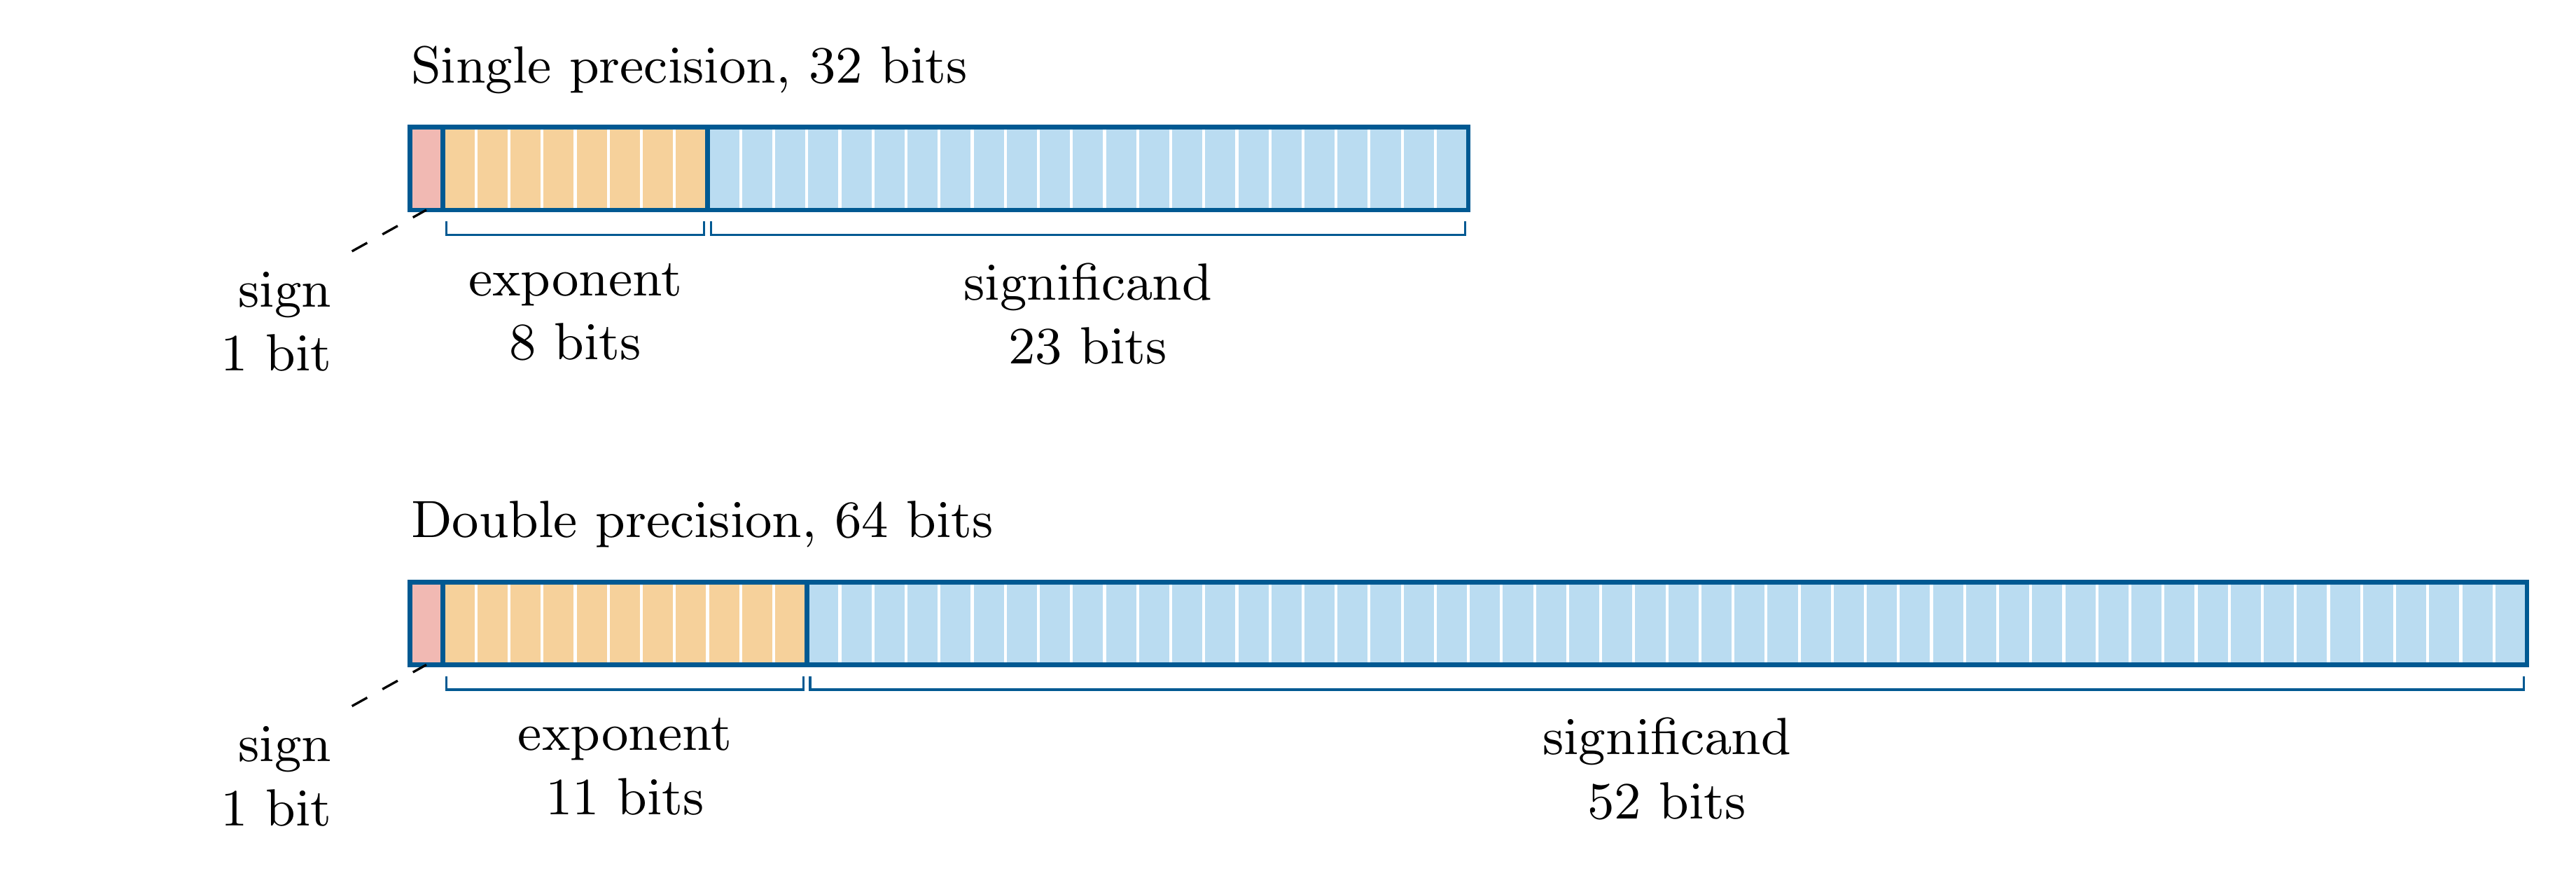
\includegraphics[width=\textwidth]{ieee754_layout.png}
\caption{IEEE 754 bit layouts. Each cell is one bit, and the bits are stored in the order sign, exponent, significand.}
\label{fig:ieee-layout}
\end{figure}

For single precision, the 8 exponent bits can represent integers up to $M = 127$, so
the largest float in single precision is roughly $10^{38}$. Double precision is the standard used in modern computers. 

\begin{Exercise}[title={Bit Allocation}, label={ex:bit-allocation}]
A floating-point system uses $N = 16$ bits total. The sign takes 1 bit and the
significand takes 10 bits.
\begin{enumerate}
    \item How many bits are left for the exponent?
    \item Five bits give $2^5 = 32$ different exponents. If they represent the integers from $-15$ to $16$, what is the
    largest exponent $M$?
    \item Would you expect this system to be more or less precise than single precision?
    Why?
\end{enumerate}
\end{Exercise}
\begin{Answer}[ref={ex:bit-allocation}]
\begin{enumerate}
    \item $16 - 1 - 10 = 5$ bits for the exponent.
    \item $M = 16$.
    \item Less precise than single precision. Single precision has $p = 23$ significand
    bits; this system has only $p = 10$, so it can store fewer digits and will produce
    larger roundoff errors.
\end{enumerate}
\end{Answer}

\subsubsection{Machine Epsilon}

The \newterm{machine epsilon}\index{machine epsilon} is commonly written as $u$. It measures the largest relative gap between a real number and
its nearest float. In other words, it tells you the worst-case precision of your
system.

For a system that rounds to the nearest float, machine epsilon is
\[
    u = \frac{1}{2} \beta^{1-p},
\]
where $\beta$ is the base and $p$ is the precision. In IEEE 754, every nonzero binary significand starts with a 1, so that
bit is not stored: double precision keeps 52 bits but has precision $p = 53$
(single precision: 23 stored, $p = 24$). For double precision, $\beta = 2$ and
$p = 53$, giving $u = 2^{-53} \approx 1.11 \times 10^{-16}$. That means any
real number is stored with a relative error no worse than about $1.1 \times
10^{-16}$: roughly 16 significant decimal digits of accuracy.

If you have access to Python, you can check your machine epsilon directly (\index{sys.float\_info}):

\begin{minted}{python}
import sys
print(sys.float_info.epsilon)   # double precision machine epsilon
\end{minted}

Every machine running IEEE 754 double precision should return the same value:
\texttt{2.220446049250313e-16}. This is twice the value of $u$ above: Python reports the gap between $1$ and the next float, $2^{-52}$, while $u$ is half a gap, because rounding to the nearest float is never off by more than half the gap.

\begin{Exercise}[title={Machine Epsilon}, label={ex:machine}]
A base-10 floating-point system has precision $p = 6$ and uses rounding.
\begin{enumerate}
    \item Compute machine epsilon $u$ for this system.
    \item A real number $x$ is stored as a float $\tilde{x}$. Using your answer above,
    what is the worst-case relative error $\frac{|\tilde{x} - x|}{|x|}$?
    \item If $p$ were doubled to $p = 12$, how would $u$ change?
\end{enumerate}
\end{Exercise}
\begin{Answer}[ref={ex:machine}]
\begin{enumerate}
    \item $u = \frac{1}{2} \times 10^{1-6} = \frac{1}{2} \times 10^{-5} = 5 \times
    10^{-6}$.
    \item The worst-case relative error is $u = 5 \times 10^{-6}$, meaning about 6
    significant digits of accuracy.
    \item $u = \frac{1}{2} \times 10^{1-12} = 5 \times 10^{-12}$. Doubling the
    precision shrinks machine epsilon by a factor of $10^6$.
\end{enumerate}
\end{Answer}

\textbf{Good to know:} IEEE 754 has been updated since 1985. The current standard includes
\newterm{quadruple precision}\index{quadruple precision} (128 bits) for applications
that need the highest accuracy. This includes physics simulations and cryptographic
computations. Whole numbers can also be stored in integer types, such as \texttt{int32} and \texttt{int64}. Use them when you only need whole numbers, since integer arithmetic avoids the rounding error of floating-point arithmetic. 

The existence of multiple precisions is a reminder that there is always a trade-off.
More bits means more accuracy and a wider range, but also more memory and slower
computation. Choosing the right precision for a given problem is the real engineering
decision.


\section{Data Compression and Decompression}
Data compression and decompression are fundamental techniques used in
modern computing, enabling efficient storage and transmission of
data. The concept of entropy, borrowed from the field of information
theory, plays a crucial role in determining the compression rate.\index{data compression}

Data compression is the process of reducing the amount of data needed
to represent a particular set of information. The two main types of
data compression are lossless and lossy. Lossless compression ensures
that the original data can be perfectly reconstructed from the
compressed data, whereas lossy compression allows some loss of data
for more significant compression rates.
\index{lossy}\index{lossless}
\index{decompression}Decompression is the reverse process of compression, reconstructing
the original data from the compressed format.

\subsection{Entropy}\index{information theory}

In information theory, entropy measures the unpredictability or
randomness of information content. More specifically, it quantifies
the expected value of the information contained in a message. Lower
entropy implies less randomness and more repetitiveness, which in turn
means the data can be compressed more.\index{entropy}

\subsection{Entropy and Compression}\index{entropy!compression rate}

The role of entropy in data compression is fundamental. The entropy of
a source of data is the minimum number of bits required, on average,
to encode symbols drawn from the source. It serves as a lower bound on
the best possible lossless compression rate.

For a source $X$ with \index{entropy!formula} probability distribution $p(x)$, the entropy $H(X)$ is defined as:

\begin{equation}
H(X) = - \sum_{x \in X} p(x) \log_2 p(x)
\end{equation}

If the entropy of the data is high (i.e., the data is random and
unpredictable), the potential for compression is low. On the other
hand, if the entropy is low (the data is predictable), the data can be
compressed to a smaller size.

\textbf{Worked example.} A fair coin flip has $p(\text{heads}) = p(\text{tails}) = \frac{1}{2}$:
$$H = -\left(\tfrac{1}{2}\log_2\tfrac{1}{2} + \tfrac{1}{2}\log_2\tfrac{1}{2}\right) = 1 \text{ bit}$$
No scheme can store a long run of fair coin flips in less than 1 bit per
flip. But a coin that lands heads 90\% of the time has
$$H = -(0.9\log_2 0.9 + 0.1\log_2 0.1) \approx 0.47 \text{ bits}$$
so a long record of its flips can be squeezed to less than half a bit per
flip. Predictable data compresses well.

\begin{Exercise}[title={Entropy of a Message}, label={ex:entropy}]
A source sends the letter A half the time, and B and C a quarter of the
time each. Compute its entropy. Then show that the code A = \texttt{0},
B = \texttt{10}, C = \texttt{11} achieves it.
\end{Exercise}
\begin{Answer}[ref={ex:entropy}]
$$H = -\left(\tfrac{1}{2}\log_2\tfrac{1}{2} + \tfrac{1}{4}\log_2\tfrac{1}{4} + \tfrac{1}{4}\log_2\tfrac{1}{4}\right) = \tfrac{1}{2}(1) + \tfrac{1}{4}(2) + \tfrac{1}{4}(2) = 1.5 \text{ bits}$$
The code uses 1 bit half the time and 2 bits the other half, an average of
$\frac{1}{2}(1) + \frac{1}{2}(2) = 1.5$ bits per letter, which matches the
entropy. (Because no code word is the start of another, the bits can be
decoded without spaces: \texttt{01011} is A, B, C.)
\end{Answer}
